\documentclass{article}
\usepackage{amsmath}
\usepackage{tikz}
\usetikzlibrary{positioning}

\begin{document}

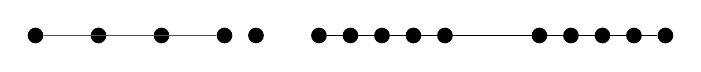
\begin{tikzpicture}[scale=0.8, every node/.style={circle, inner sep=2pt, fill=black}]
    \node (v1) at (-4,0) {};
    \node (v2) at (-3,0) {};
    \node (v3) at (-2,0) {};
    \node (v4) at (-1,0) {};
    \node (v5) at (-0.5,0) {};
    
    \draw[red] (v1) -- (v3);
    \draw[red] (v2) -- (v4);
    
    \node (v6) at (0.5,0) {};
    \node (v7) at (1,0) {};
    \node (v8) at (1.5,0) {};
    \node (v9) at (2,0) {};
    \node (v10) at (2.5,0) {};
    
    \draw[red] (v6) -- (v8);
    \draw[red] (v7) -- (v9);
    
    \node (v11) at (4,0) {};
    \node (v12) at (4.5,0) {};
    \node (v13) at (5,0) {};
    \node (v14) at (5.5,0) {};
    \node (v15) at (6,0) {};
    
    \draw (v6) -- (v10);
    \draw (v7) -- (v11);
    \draw (v8) -- (v12);
    \draw (v9) -- (v13);
    \draw (v10) -- (v14);
    \draw (v11) -- (v15);
\end{tikzpicture}

\end{document}